\documentclass[journal=jpcbfk]{achemso}

\usepackage[version=3]{mhchem}
\usepackage[T1]{fontenc}
\newcommand*\mycommand[1]{\texttt{\emph{#1}}}
\newcommand{\todo}[1]{\textcolor{red}{#1}}

\usepackage{upgreek}				
\usepackage{xcolor}
\usepackage{booktabs}
\usepackage{multirow}
\usepackage{lmodern}
\usepackage{microtype}


\author{Josef Melcr}
\author{Hector Martinez-Seara}
\affiliation{Institute of Organic Chemistry and Biochemistry,
Academy of Sciences of the Czech Republic, 
Prague 6, Czech Republic}
\author{Ji{\v r}{\' i} Kolafa}
\affiliation{Department of Physical Chemistry, Institute of Chemical Technology, Prague 6, Czech Republic}
\author{Pavel Jungwirth}
\affiliation{Institute of Organic Chemistry and Biochemistry,
Academy of Sciences of the Czech Republic, 
Prague 6, Czech Republic}
\alsoaffiliation{Department of Physics, Tampere University of Technology, P.O. Box 692, FI-33101
Tampere, Finland}

\author{O. H. Samuli Ollila}
\email{samuli.ollila@helsinki.fi}
%\homepage[]{Your web page}
\affiliation{Institute of Organic Chemistry and Biochemistry,
Academy of Sciences of the Czech Republic, 
Prague 6, Czech Republic}
\alsoaffiliation{Institute of Biotechnology, University of Helsinki}




\SectionNumbersOn

\renewcommand{\thetable}{S\arabic{table}}%
\renewcommand{\thefigure}{S\arabic{figure}}%
\renewcommand{\thesection}{S\arabic{section}}%
\renewcommand{\thepage}{S\arabic{page}}%

\title{Supporting Information:\\Accurate binding of sodium and calcium to phospholipid bilayers by effective inclusion of electronic polarization}

\begin{document}

\newpage
%\tableofcontents

\section{Simulation details}

\begin{table}[!h]
  \caption{Simulation parameters}
  \label{tbl:mdpar}
  \begin{tabular}{ll}
    simulation property & parameter   \\
    \hline
    time-step           & 2~fs         \\
    equilibration time  & 100~ns  \\
    total simulation time     & 300~ns  \\
    temperature         & 313~K       \\
    thermostat          & v-rescale  \cite{bussi07}   \\
    barostat            & Parrinello-Rahman, semi-isotropic \cite{parrinello81} \\
    long-range electrostatics & PME  \cite{darden93}  \\
    cut-off scheme      & Verlet \cite{Pall13}      \\
    Coulomb and VdW cut-off & 1.0~nm \\
    constraints         & LINCS, only hydrogen atoms \cite{hess97} \\
    constraints for water & SETTLE  \cite{miyamoto92} \\
    \hline
  \end{tabular}
\end{table}


\section{Area per molecule and calcium binding with different water models}

\begin{table}[!h]
  \caption{Area per lipid (APL) from different models of POPC with no ions\label{tab:apls_si} }
  \begin{tabular}{l|c c}
    model          & APL (\AA$^2$)   & Temperature [K] \\
    \hline
    Lipid14                   & 65.1$\pm$ 0.6  &  300 \\
    Lipid14 \cite{dickson14}  & 65.6$\pm$ 0.5  &  303 \\
    \hline
    ECC-lipids &        &  \\
    %Lipid14ecc0.80+sigma0.875 &        &  313    \\
    %($4.6\cdot 5.1 \, \mathrm{nm}^2$), 72 lipids patch, OPC3           & 63.2   &   313      \\
    ~ OPC3           & 62.2$\pm$ 0.6   &  300       \\
    ~ OPC3           & 64.2$\pm$ 0.6   &  313       \\
    ~ SPC/E          & 65.1$\pm$ 0.6   &  313       \\
    ~ SPC/E          & 63.2$\pm$ 0.6   &  300       \\
    ~ OPC            & 64.4$\pm$ 0.6   &  313       \\
    ~ TIP4p/2005     & 66.8$\pm$ 0.6   &  313       \\
    ~ TIP3p          & 66.2$\pm$ 0.6   &  313       \\
    ~ TIP3p-FB       & 64.8$\pm$ 0.6   &  313       \\
    ~ TIP4p-FB       & 65.6$\pm$ 0.6   &  313       \\
    %($9.2\cdot 10.2 \, \mathrm{nm}^2$), 288 lipids patch           & 65.5   &  313       \\ %% not done for this model with f_sigma=0.89
    %oMM small patch           & 63.65  &         \\
    %oMM 4xbig patch           & 63.7   &         \\
    \hline
    experiment   & 62.7  &  293    \\
    experiment \cite{kucerka11} & 64.3  &  303    \\
    experiment  & 67.3  &  323    \\
    experiment  & 68.1  &  333    \\
    %experiment POPE  & 56.6 &  303    \\
    \hline
  \end{tabular} \\
\end{table}


\begin{figure}[!h]
  \centering
  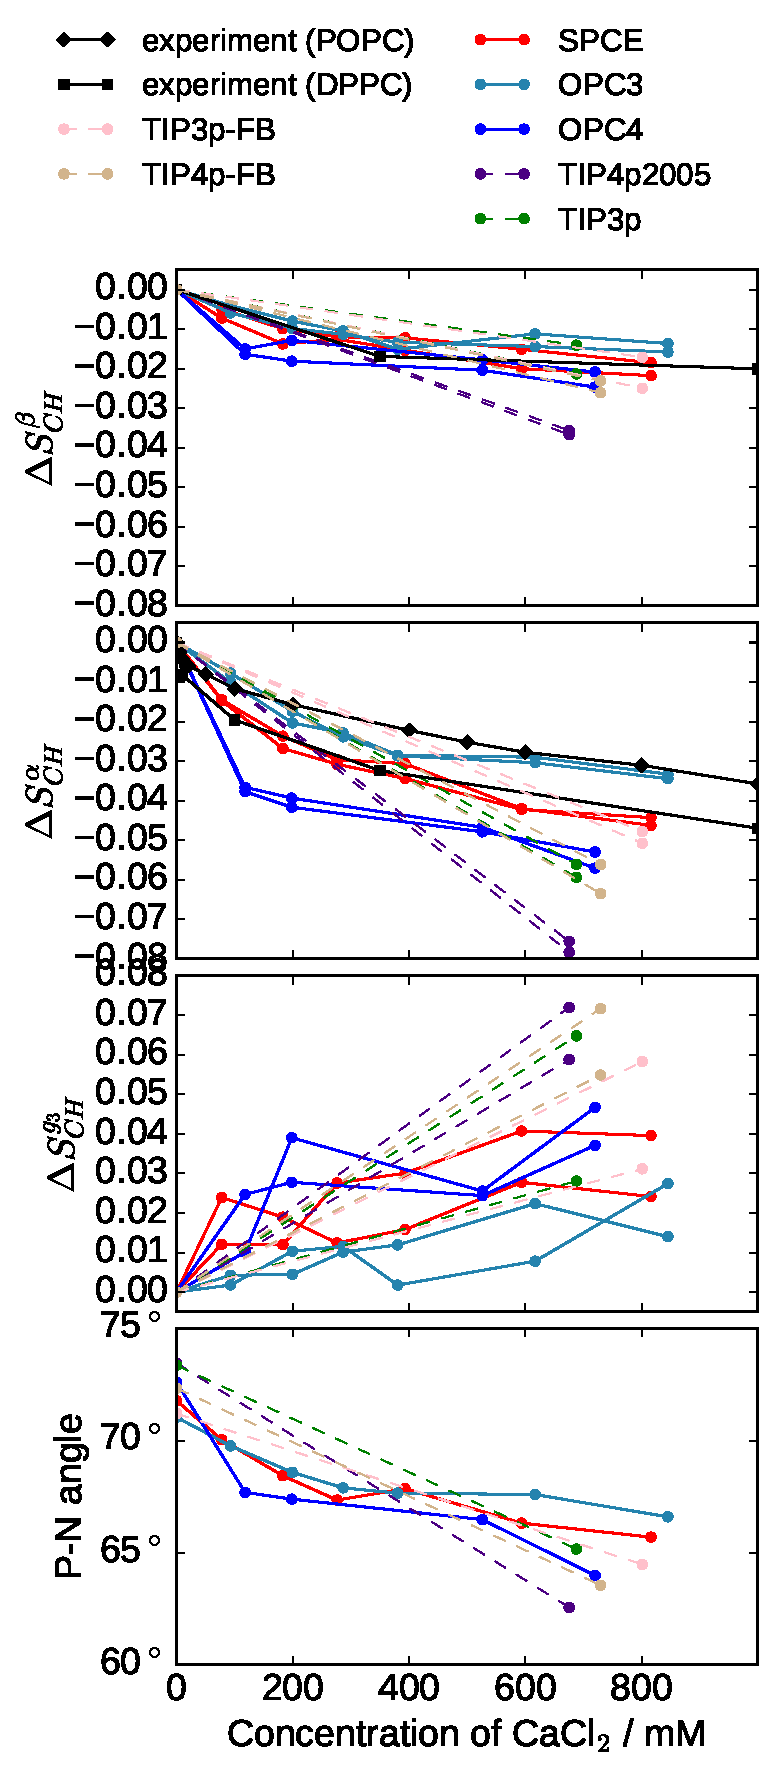
\includegraphics[width=8.0cm]{../Fig/ipython_nb/PN_angle_OrdPars-A-B-g3_L14-ECCL17_q80_sig89_CaCl_waterModels.pdf}
  \caption{\label{fig:ordPars_waterModels}
    Changes of head group order parameters of POPC bilayer as a function of CaCl$_2$ concentrations
    are shown from simulations with different force fields and water models together with experimental data 
    (DPPC \cite{akutsu81} and POPC \cite{altenbach84}). 
    Ion concentrations in bulk water are shown in x-axis. 
    Values from simulations are calculated from the of cation number density $C_{np}$
    from the region at the simulatin box edge with the constant ion concentration as [ion]=$C_{np}/0.602$.
  }
\end{figure}

\section{Sodium binding to POPC with the glycerol carbon and changes in the head group angle}

\begin{figure}[!h]
  \centering
  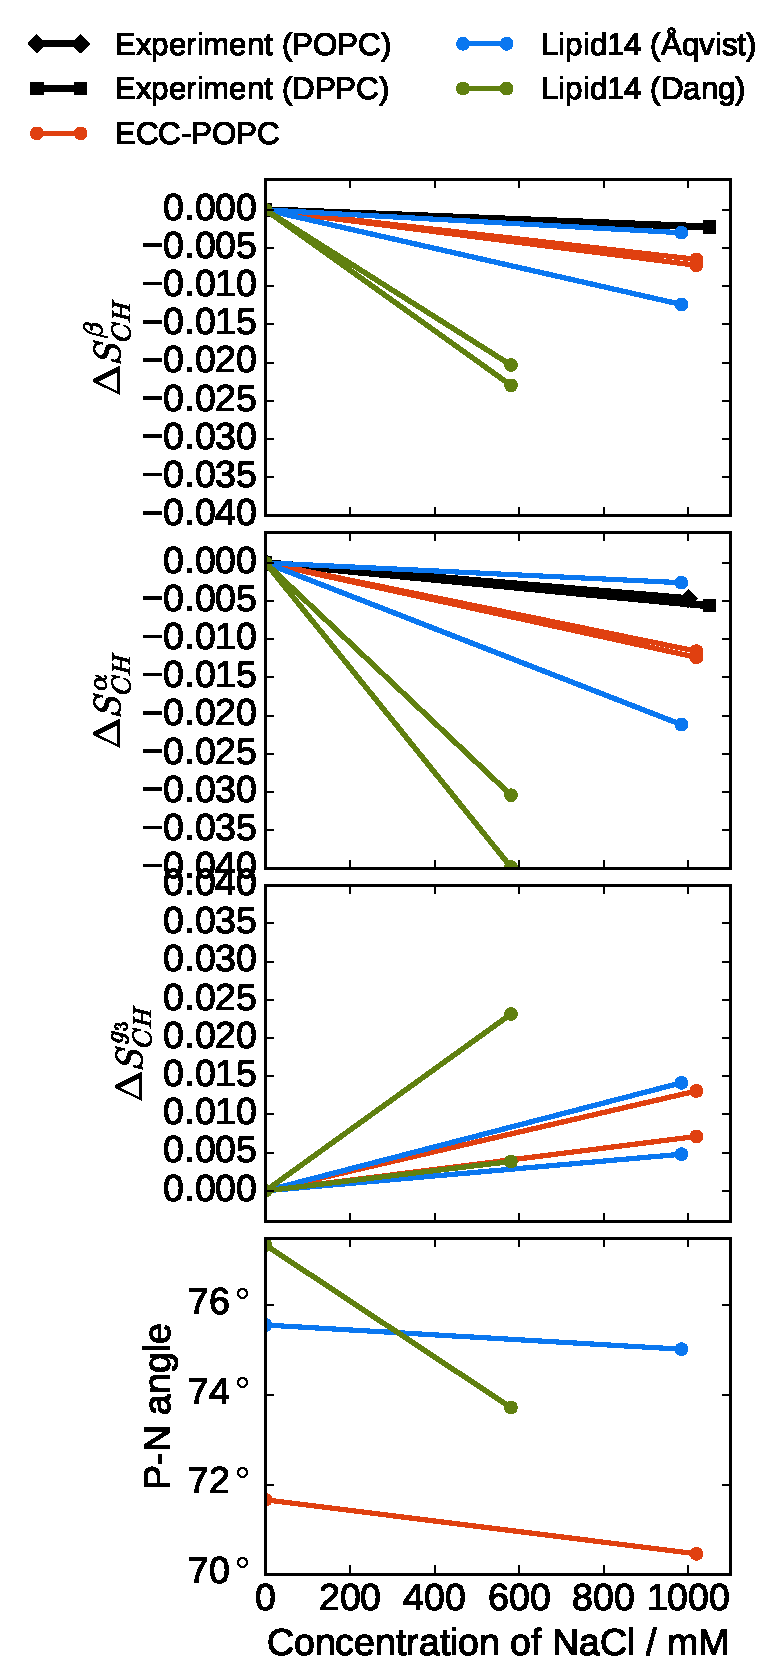
\includegraphics[width=8.0cm]{../Fig/ipython_nb/PN_angle_OrdPars-A-B-g3_L14-ECCL17_q80_sig89_NaCl.pdf}
  \caption{\label{fig:delta_ordPar_NaCl_si}
    Changes of head group and glycerol $g_3$ order parameters and the P-N vector angle of POPC bilayer as a function of NaCl concentrations
    from simulations with different force fields together with experimental data \cite{akutsu81}. 
    Ion concentrations in bulk water are shown in x-axis. 
%    Values from simulations are calculated from the of cation number density $C_{np}$
%    from the region at the simulatin box edge with the constant ion concentration as [ion]=$C_{np}/0.602$.
    Simulation data with Lipid14 and \AA{}qvist ion parameters is taken directly from Ref. \cite{catte16}.
  }
\end{figure}

\section{Histograms of residence times}

\begin{figure}[!h]
  \centering
  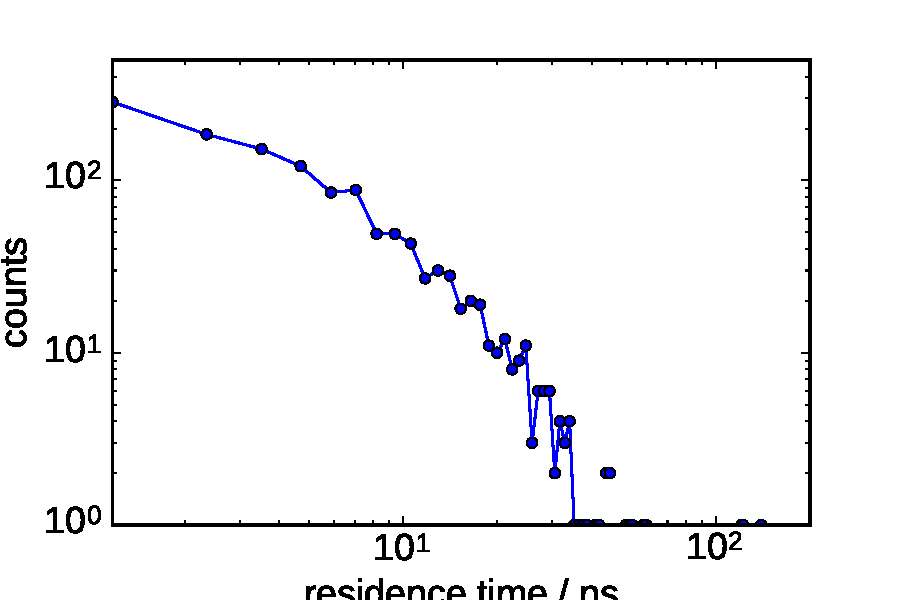
\includegraphics[width=8.0cm]{../Fig/ipython_nb/histogram_bound_times_ECC-lipids_346mM_CaCl.pdf} \\
  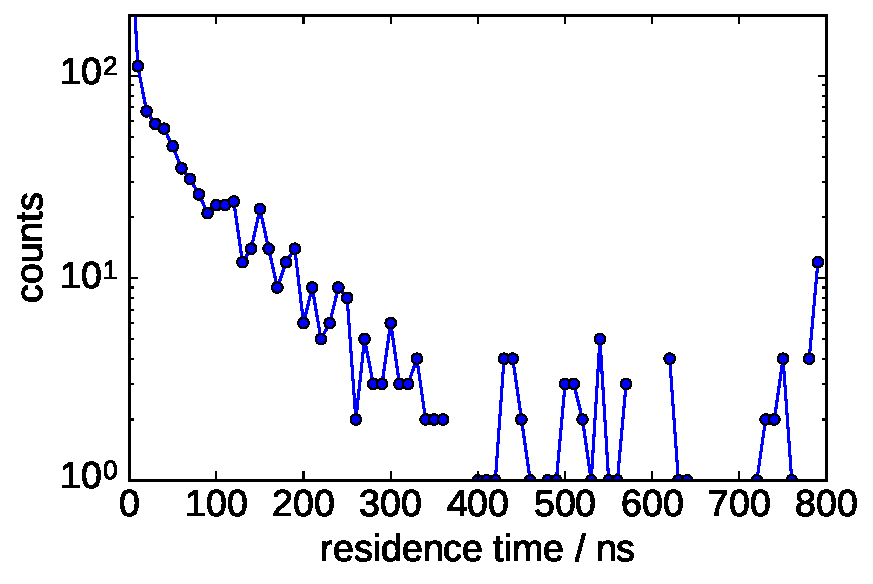
\includegraphics[width=8.0cm]{../Fig/ipython_nb/histogram_bound_times_Charmm36_450mM_CaCl_Matti.pdf}
  \caption{\label{fig:hist_residence_times}
   Histograms of residence times of \ce{Ca^{2+}} in a POPC bilayer 
   at $450\,\mathrm{mM}$ concentration of \ce{CaCl_2} in water before adsorption to phospholipids
   from simulations with ECC-lipids/ECC-ions (top)
   and CHARMM36/ECC-ions (bottom), which was taken from previous study \cite{javanainen17} 
   (simulation data available at Ref.~\citenum{zenodo.259376}).
   The maxima on the x-axis represent the lengths of the simulations used for analysis. 
   For the ECC-lipids model, 90\% of the residence times of \ce{Ca^{2+}} in a POPC membrane are 
   shorter than $60\,\mathrm{ns}$, % exactly $53\,\mathrm{ns}$
   with the longest observed residence time being $141\,\mathrm{ns}$, 
   which is well below the total length of the simulation (200~ns).
   This is, however not true for the simulation with CHARMM36 model,
   where there are several calcium cations with their residence time 
   apparently limited by the length of the simulation. 
   With such a simulation, which is relatively short for the employed model,
   we can merely estimate an upper bound that 
   only less than 60\% of the bound residence time 
   is formed by cations interacting with the phospholipid membrane 
   for less then half of the simulation length~(400~ns).
  }
\end{figure}

\section{Ternary complex model in simulations}
It was found in the original work~\cite{altenbach84} that 
a ternary complex binding model (i.e.~2~POPC:1~\ce{Ca^{2+}})
provides the best fit to experimental measurements of all considered models in that study. 
In such a model, there is a linear relationship between quantities 
$C_b$, mole fraction of bound \ce{Ca^{2+}} per POPC, and $\sqrt{C_b/C_I}$, 
where $C_I$ is the concentration of free cations at the plane of ion binding~\cite{altenbach84}.
The concentration $C_b$ was obtained from an extrapolation of linear relation 
between deuterium NMR measurements and atomic absorption spectroscopy for low concetrations of \ce{CaCl2}.
Such an extrapolation is valid as long as the mode of \ce{Ca^{2+}} binding 
remains constant throughout the extrapolation range. 
The concentration $C_I$ is determined from the surface potential using the Boltzmann equation.
However, Boltzmann theory yields inaccurate results
for divalent cations like \ce{Ca^{2+}}~\cite{Andelman1995}. 
An atomistic simulation, on the other hand, provides these quantities directly without severe assumptions;
$C_b$ can be calculated from simulation using the robust definition in section~\ref{sec:affinity},
and $C_I$ can be obtained from the density profiles in Fig.~\ref{fig:cacl-density} 
as the minimum concentration at the shallow depression separating the bulk water phase 
and the peak of adsorbed cations around 2.6\,nm from the membrene centre. 
The small discrepancy between the results in the experiment~\cite{altenbach84} and 
our simulations are likely caused by the difference in the evaluation of the concentrations. 


\begin{figure}[!h]
  \centering
  \includegraphics[height=9.0cm,angle=-90]{../Fig/bound-CAs_conc-eccl17.eps}
  \caption{\label{fig:cacl-bind}
    Ternary complex binding model of \ce{Ca^{2+}} to a POPC membrane 
    that assumes the stoichiometry of 2~POPC:1~\ce{Ca^{2+}} (details in reference~\citenum{altenbach84}) 
    provides a good fit to experimental measurements~\cite{altenbach84}
    and it also provides a good fit to our simulation data. 
    This supports our statement that the success of the ternary complex model in the experiments
    can be understood with the atomistic detail of our simulations as an average 
    stoichiometry of otherwise almost evenly distributed clusters of one cation with 1,2 or 3 lipids (Fig.~\ref{fig:cacl_complexes}). 
    Note that the units in the reference~\citenum{altenbach84} are different from the units presented here,
    and, hence, the observed slope of the linear relationship is slightly different.
    }
\end{figure}


\section{Comparison between Gromacs and openMM}

\begin{figure}[!h]
  \centering
  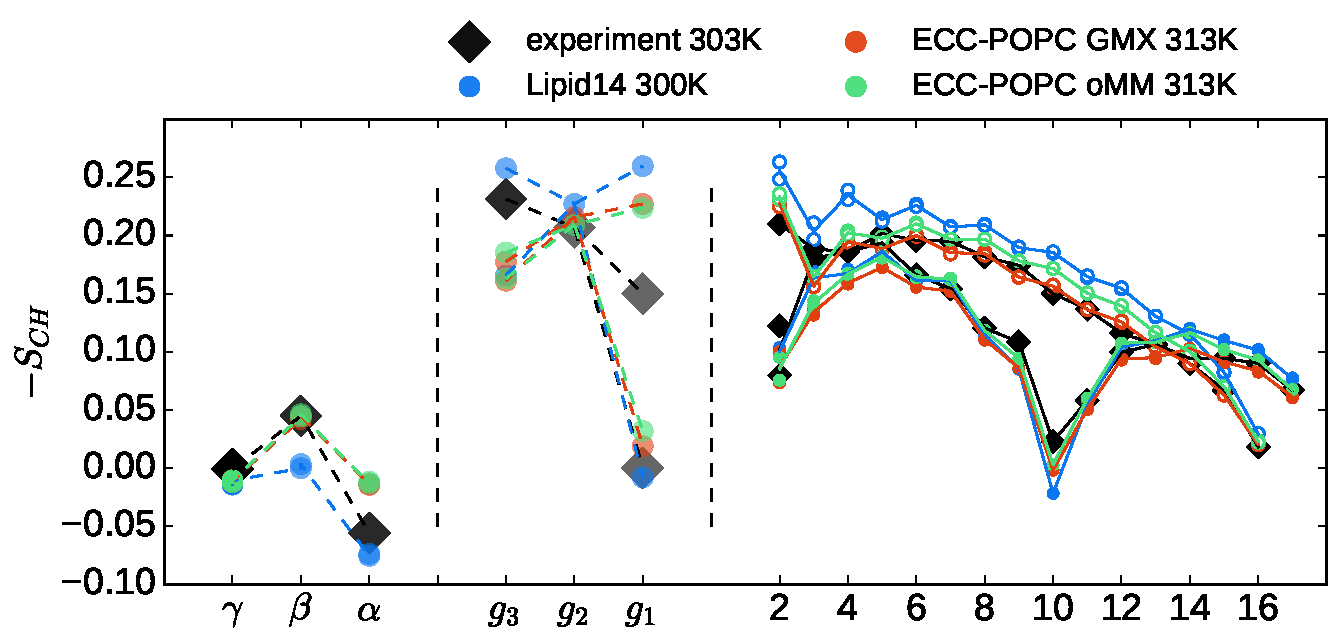
\includegraphics[width=16.0cm]{../Fig/ipython_nb/Order-parameters_exp-L14-ECCL17_q80_sig89_GMX-oMM_compar.pdf}
  \caption{\label{fig:ordPars_actual_GMX_oMM_compar}
    Order parameters of POPC head group, glycerol backbone and acyl chains 
    from simulations with the Lipid14 \cite{dickson14} and the ECC-lipids models
    simulated with GROMACS~5.1.4 \cite{Abraham15} and openMM~7 \cite{openmm7} 
    compared with the experimental values from \cite{ferreira13}.
    The size of the markers for the head group order parameters correspond to
    the error estimate $\pm 0.02$ for experiments \cite{botan15,ollila16},
    while the error estimate for simulations is $\pm 0.005$.
    The size of the points for acyl chains are decreased by a factor of 3 to improve the clarity of the plot.
  }
\end{figure}

\begin{figure}[!p]
  \centering
  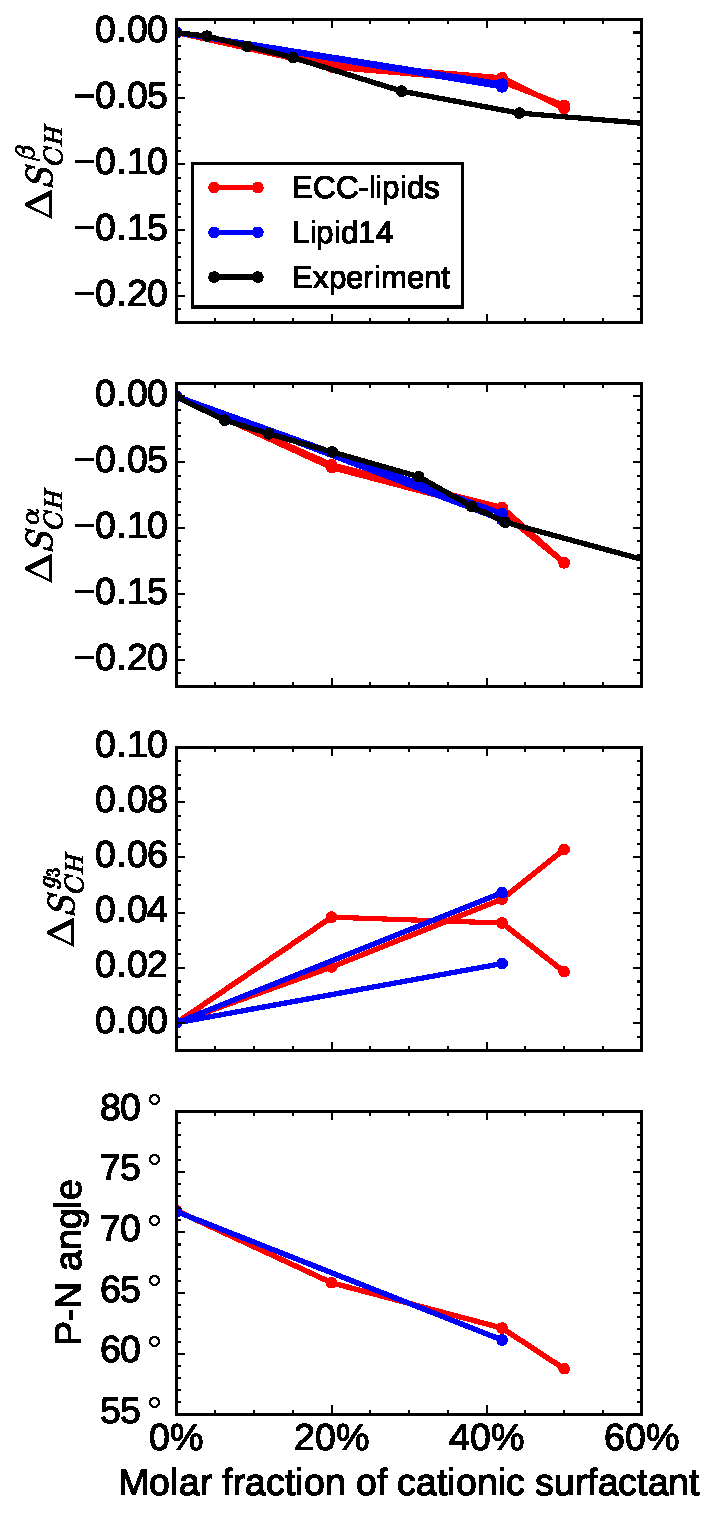
\includegraphics[width=8.0cm]{../Fig/ipython_nb/PN_angle_OrdPars-A-B-g3_L14-ECCL17_q80_sig89_surf_GMX-oMM_compar.pdf}
  \caption{\label{fig:ordPars_surf_GMX_oMM_compar}
    The changes of headgroup order parameters and P-N vector orientation as a function of
    a molar fraction of the cationic surfactant dihexadecyldimethylammonium in a POPC bilayer
    from simulations with the ECC-lipids models
    simulated with GROMACS~5.1.4 \cite{Abraham15} and openMM~7 \cite{openmm7} 
    compared with the experimental values from \cite{scherer89}.
    The size of the markers for the head group order parameters correspond to
    the error estimate $\pm 0.02$ for experiments \cite{botan15,ollila16},
    while the error estimate for simulations is $\pm 0.005$.
  }
\end{figure}

\begin{figure}[!p]
  \centering
  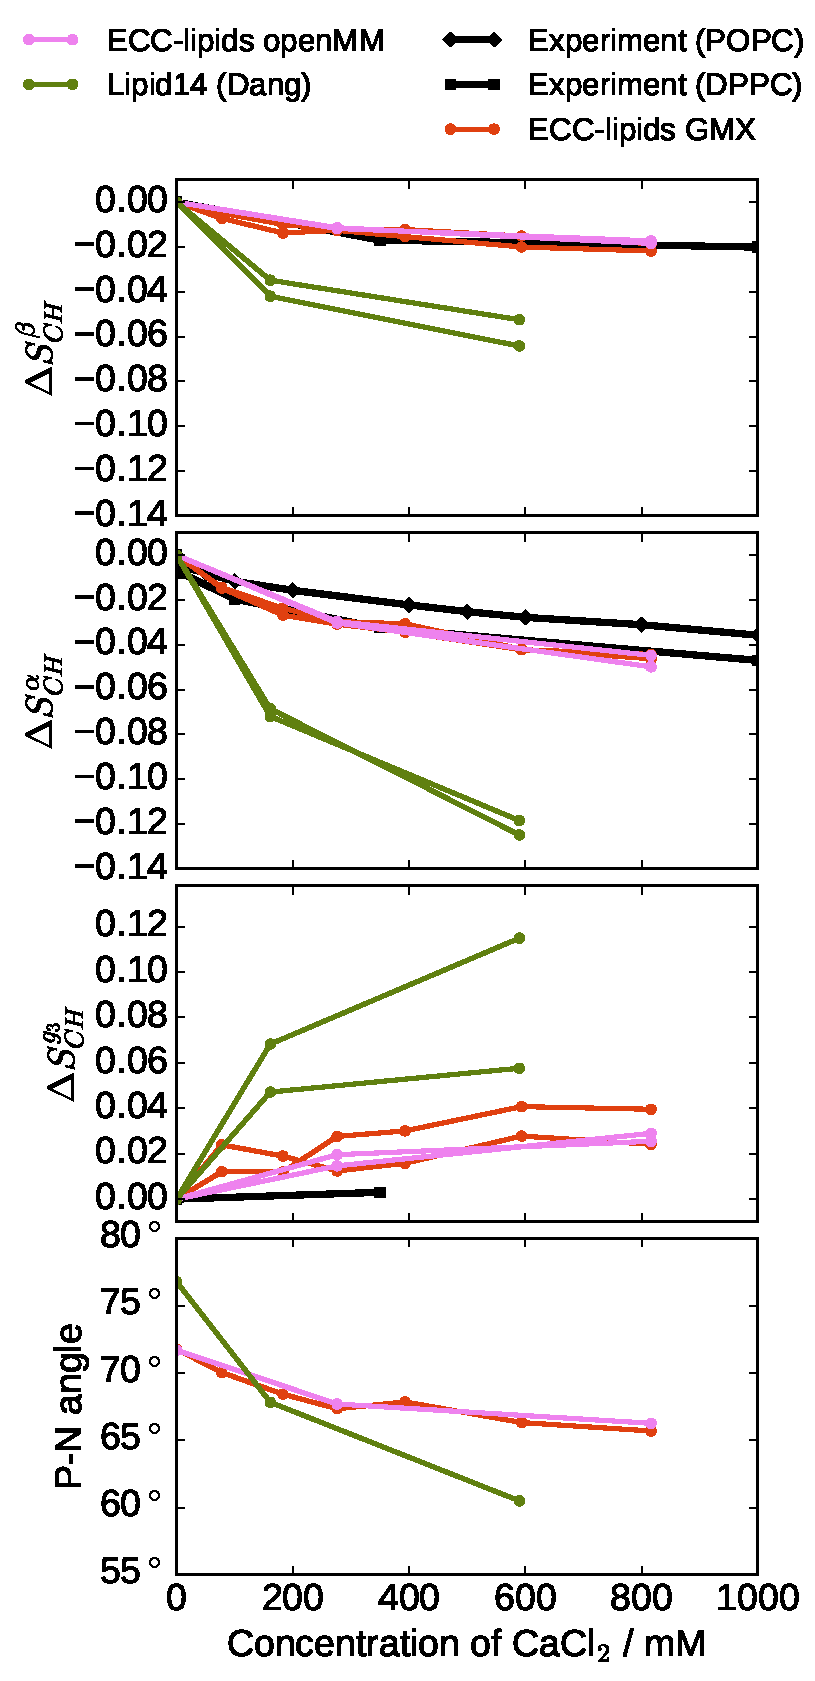
\includegraphics[width=8.0cm]{../Fig/ipython_nb/PN_angle_OrdPars-A-B-g3_L14-ECCL17_q80_sig89_CaCl_GMX-oMM_compar.pdf}
  \caption{\label{fig:ordPars_cacl_GMX_oMM_compar}
    Changes of the head group order parameters and P-N vector orientation of a POPC bilayer 
    as a function of the CaCl$_2$ concentration
    from simulations with the Lipid14 \cite{dickson14} and the ECC-lipids models
    simulated with GROMACS~5.1.4 \cite{Abraham15} and openMM~7 \cite{openmm7} 
    (DPPC (323\,K) \cite{akutsu81} and POPC (313\,K) \cite{altenbach84}). 
    Ion concentrations in bulk water are shown in x-axis. 
    Bulk concentrations from simulations are calculated 
    from the farthest point from the lipid bilayer in the aqueous phase
    with an error estimate of 10\,mM.
  }
\end{figure}



\newpage
\bibliography{refs.bib}

\end{document}
